\documentclass[border=3pt,tikz]{standalone}
\usepackage{amsmath,amssymb}
\usepackage{bm}
\usepackage{tikz}
\usetikzlibrary{patterns}
\tikzset{>=stealth}

\colorlet{mygreen}{teal!80!black}
\colorlet{myviolet}{blue!70!black}

\begin{document}

% VELOCITY vs. TIME
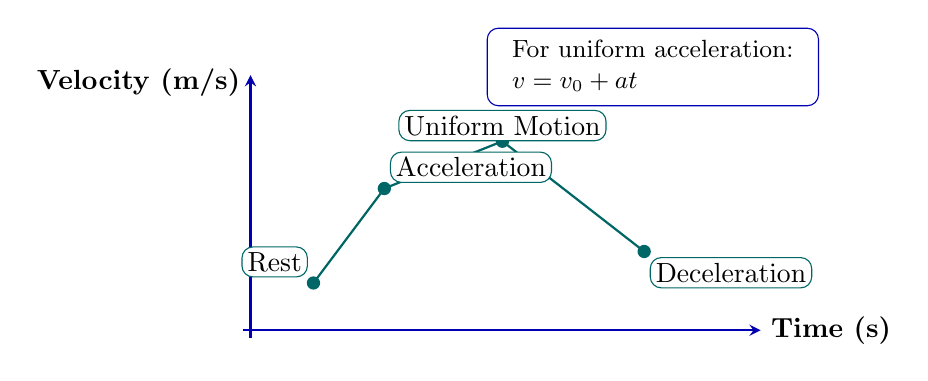
\begin{tikzpicture}
  \def\xMin{-0.1} \def\xMax{6.0}
  \def\yMin{-0.1} \def\yMax{3.0}
  
  % Coordinates for the line graph
  \coordinate (A) at (0.8,0.6);   % Initial (Rest)
  \coordinate (B) at (1.7,1.8);   % Acceleration
  \coordinate (C) at (3.2,2.4);   % Constant velocity
  \coordinate (D) at (5.0,1.0);   % Deceleration

  % Draw axes
  \draw[->,thick,myviolet]
    (\xMin,0) -- (1.08*\xMax,0) node[right,black] {\textbf{Time (s)}};
  \draw[->,thick,myviolet]
    (0,\yMin) -- (0,1.08*\yMax) node[above=6pt,below left,align=center,black] {\textbf{Velocity (m/s)}};

  % Draw the main line graph
  \draw[thick,mygreen,line join=round]
    (A) -- (B) -- (C) -- (D);

  % Dots at data points
  \foreach \pointName/\pointLabel in {A/Start, B/Accelerate, C/Uniform, D/Stop}
    \fill[mygreen] (\pointName) circle (2.4pt);

  % Node labels
  \node[above left=2pt,fill=white,inner sep=2pt,draw=mygreen,rounded corners] at (A) {Rest};
  \node[above right=2pt,fill=white,inner sep=2pt,draw=mygreen,rounded corners] at (B) {Acceleration};
  \node[above,fill=white,inner sep=2pt,draw=mygreen,rounded corners] at (C) {Uniform Motion};
  \node[below right=2pt,fill=white,inner sep=2pt,draw=mygreen,rounded corners] at (D) {Deceleration};

  % Example equation annotation
  \node[above=24pt,right,align=left,fill=white,draw=myviolet,rounded corners,inner sep=3pt] at (3.0,2.5)
    {\small\begin{tabular}{l}
      For uniform acceleration:\\
      $\displaystyle v = v_0 + a t$
    \end{tabular}};
\end{tikzpicture}

\end{document}
